%  Copyright (C) 2005 The Regents of the University of California.
%  Produced at Lawrence Livermore National Laboratory (cf, DISCLAIMER).
%  Written by Jim Garlick <garlick@llnl.gov>.
%  UCRL-CODE-218333
%  
%  This file is part of ISP, a toolkit for constructing pipeline applications.
%  For details, see <http://isp.sourceforge.net>.
%
%  ISP is free software; you can redistribute it and/or modify it under
%  the terms of the GNU General Public License as published by the Free
%  Software Foundation; either version 2 of the License, or (at your option)
%  any later version.
%  
%  ISP is distributed in the hope that it will be useful, but WITHOUT ANY
%  WARRANTY; without even the implied warranty of MERCHANTABILITY or FITNESS
%  FOR A PARTICULAR PURPOSE.  See the GNU General Public License for more
%  details.
%  
%  You should have received a copy of the GNU General Public License along
%  with ISP; if not, write to the Free Software Foundation, Inc.,
%  59 Temple Place, Suite 330, Boston, MA  02111-1307  USA.

\documentclass{article}

\usepackage{verbatim}
\usepackage{calc}
\usepackage{epsfig}
\input{pstricks}

\setlength{\textwidth}{6in}
\setlength{\textheight}{9in}
\setlength{\oddsidemargin}{(\paperwidth-\textwidth)/2 - 1in}
\setlength{\topmargin}{(\paperheight-\textheight -\headheight-\headsep-\footskip)/2 - 1in + .5in }

\begin{document}

\title{Industrial Strength Pipes\footnote{
	ISP is licensed under the terms of the GNU General Public License.  
	You should have received a copy of the GNU General Public License 
	along with ISP; if not, write to the Free Software Foundation, Inc.,
	59 Temple Place, Suite 330, Boston, MA  02111-1307  USA.
	This work was produced at the University of California, 
	Lawrence Livermore National Laboratory under Contract 
	No. W-7405-ENG-48 with the DOE.  
	UCRL-CODE-218333
	\copyright 2005 The Regents of the University of California.
	}\\
	Version 0.10}
\author{Jim Garlick\\ garlick@llnl.gov}

\date{Dec. 12, 2005}

\maketitle

\section{Introduction}

Industrial Strength Pipes (ISP) is a toolkit for constructing pipeline
applications using the UNIX pipe and filter model.  
In UNIX, the ``do one thing and do it well'' philosophy as applied to 
text filters is considered a big success.  ISP tries to capitalize on this
in applications that look architecturally similar to UNIX pipelines, but
require more complicated interactions between filters, such as image processing
pipelines.  Like UNIX filters, 
ISP filters can have their standard output and standard input chained
with a shell command such as:
\begin{verbatim}
foo | bar | baz >result
\end{verbatim}
Unlike UNIX filters which pass unstructured character streams or 
newline-separated lines, ISP filters pass structured information in XML 
format.  The XML contains a stream of records that are processed by
filters, analogous to the stream of lines processed by {\em grep}.

ISP is geared toward pipelines that apply a succession
of transformation algorithms to data files, producing and consuming 
metadata and files associated with the original data along the 
way\footnote{ISP has origins in astronomical image processing, though
it is designed to be general purpose.}.
ISP was designed to be simple to use and program with a familiar pipeline
construction and execution model, and yet provide a framework that allows
for advanced features to be implemented such as file management, 
strong metadata typing, parallel execution, fault tolerance, data 
provenance, and logging.

Filters obtain ISP services through an application programming 
interface (API) written in the C programming language.
The ISP package consists of the API headers and libraries and a small
collection of general-purpose filters.

\section{Anatomy of an ISP Pipeline Application}

ISP preserves the UNIX pipe and filter model as much as possible.
ISP applications are composed of filters chained together in the usual
way by a UNIX shell.  The shell is the parent of each filter and
its role is simply to set up the pipeline, block while the filters execute,
then report their completion status.  There is no additional software 
overseeing ISP application execution --- all processing is cooperative between
filters.

ISP filters read a stream of XML records from standard input, perform some
processing on each record, and emit the processed records on standard output.
The XML usually is created by a single-ended filter at the beginning of the 
pipeline, and the XML emerging from the end of the pipeline is redirected 
to a file which may be kept as a record of the processing.
Filters use standard error in the usual way to report errors and warnings.
Figure~\ref{figschematic} is a schematic depiction of an ISP pipeline.

ISP records may contain file references and simple typed metadata, 
indexed by string key.  ISP filters can be structured in more than
one way, but the simplest type of filter is the {\em map filter}.
A map filter registers a function that is called for each record read on
standard input.  The function uses ISP accessors to access and modify the 
file references and metadata in the record, then returns an integer code 
indicating success or failure.  ISP takes care of all the I/O and XML 
parsing, and also optionally skips calling the map function on records 
that have logged upstream failures.

Each filter registers a {\em symbol table} that describes the key names and 
types of the files and metadata it expects to access, add to, or remove 
from the record.  When a pipeline is run, a special handshake occurs that
terminates the pipeline if the symbol tables do not match up.  For example,
if a filter says it will access a file with key ``rawimage'', and no upstream
filter has sent a symbol table downstream that says it is providing a file 
with that key name, the filter displays a message on standard error and 
exits, which terminates the pipeline.

The overall organization of the data within each record is not known 
to the filters.  The filters just know about the data they operate on.
This allows general purpose filters to be created and 
reused in different pipelines.

%\footnote{In practice, it is difficult 
%to generalize a filter that encapsulates a complex, highly tunable algorithm.
%Such filters tend to take on application-specific assumptions like hard coded
%paramaters and checks for valid input data.  Filters that are easily 
%reusable tend to be the ones that have simple interfaces, like the 
%general purpose filters supplied with the ISP package.}

\begin{figure}
\begin{center}
 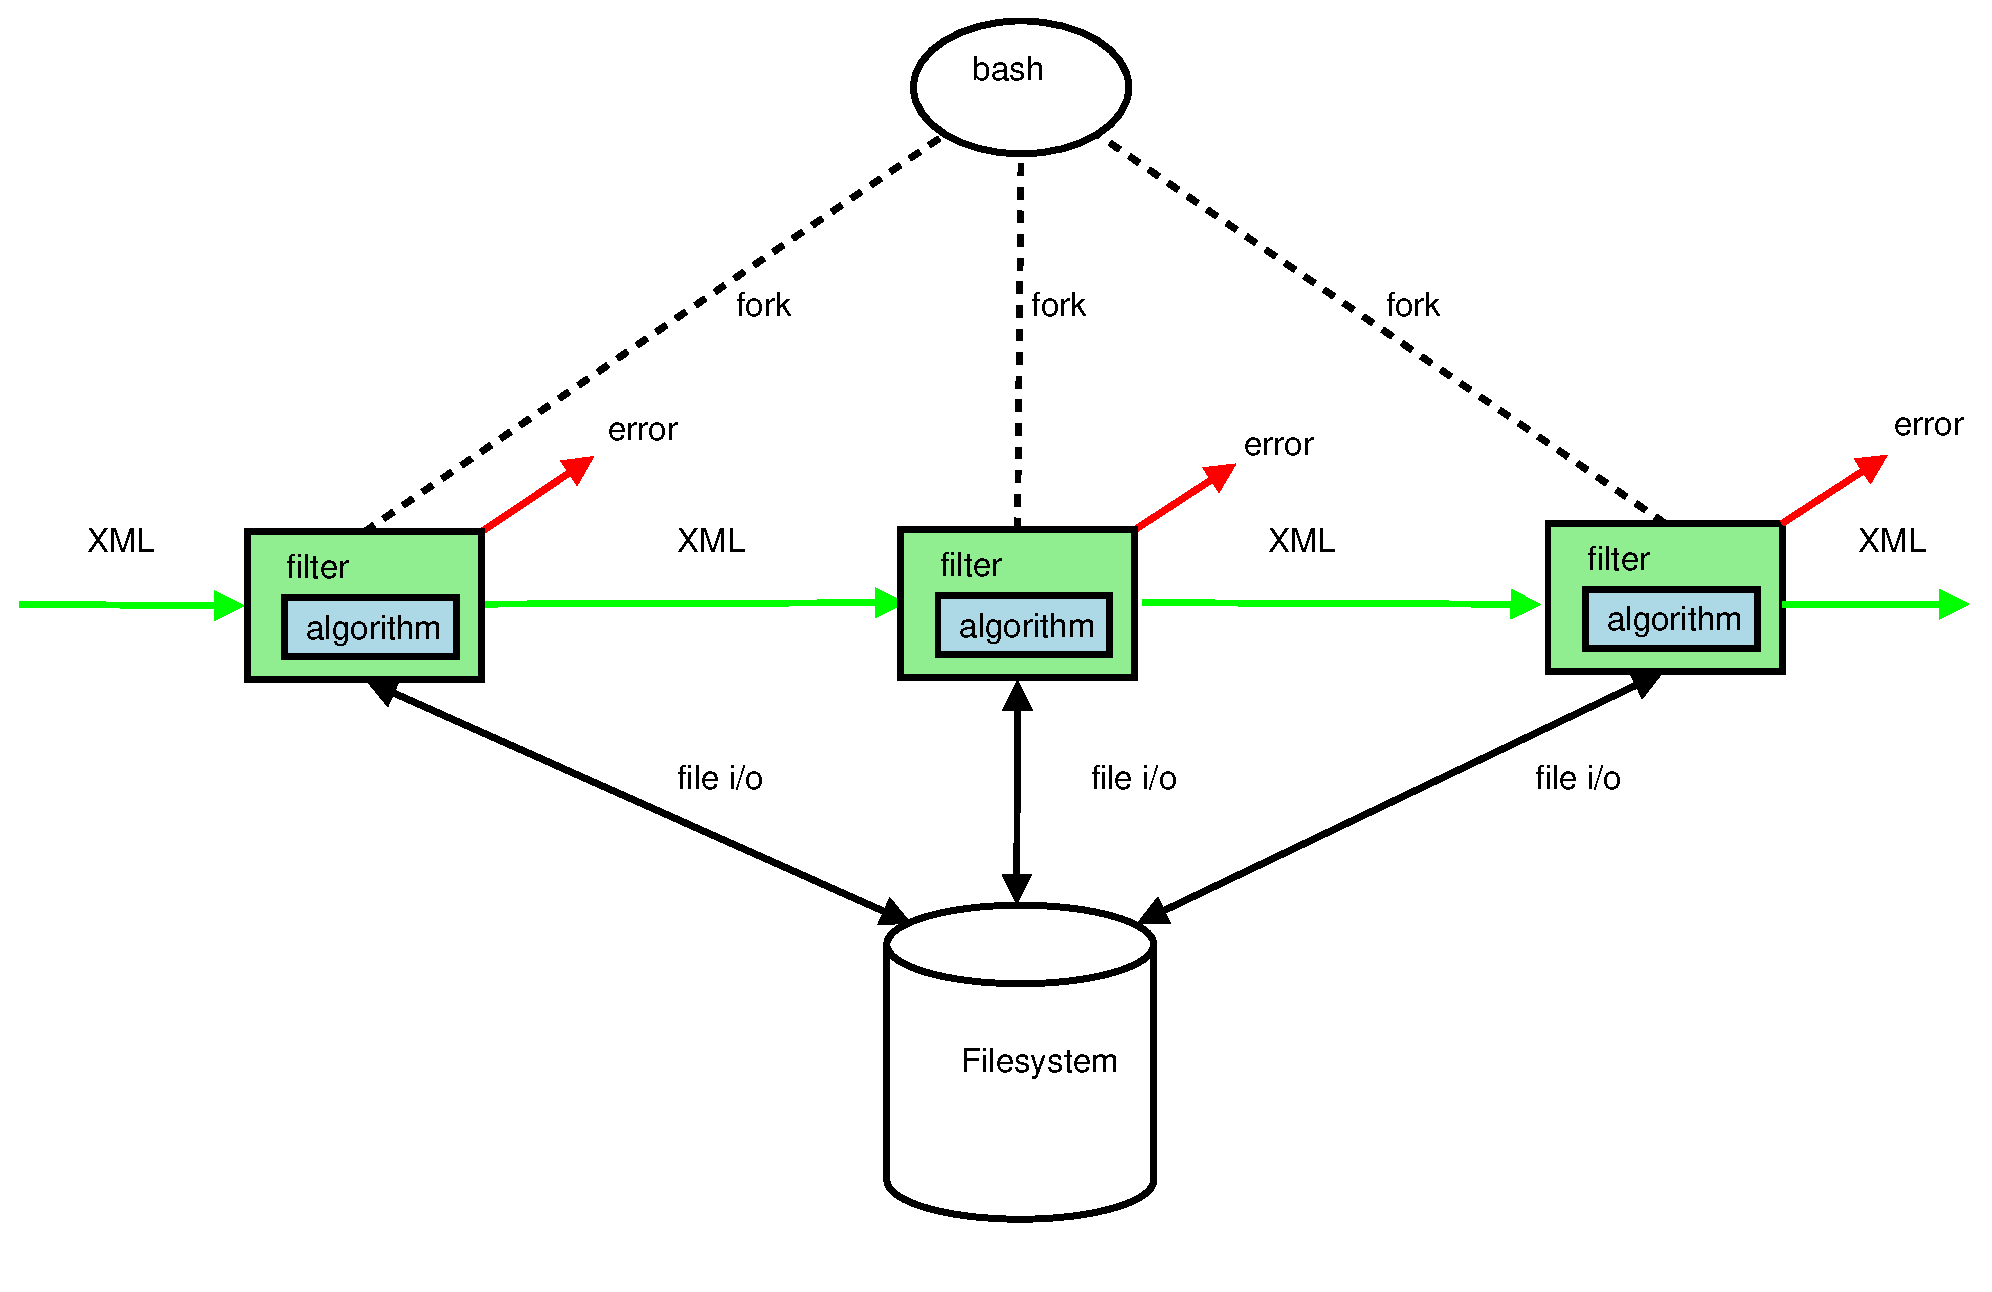
\includegraphics[width=\linewidth]{isp.eps}
\end{center}
\caption{An ISP Pipeline}\label{figschematic}
\end{figure}

\section{XML Document Structure}\label{secxml}

\begin{figure}
\begin{center}
\begin{tabular}{|l|}\hline
$<$?xml version="1.0" standalone="yes"?$>$\\
$<$document$>$\\
$<$init$>$ ... $<$/init$>$\\
$<$unit$>$ ... $<$/unit$>$\\
$<$unit$>$ ... $<$/unit$>$\\
...\\
$<$unit$>$ ... $<$/unit$>$\\
$<$/document$>$\\
\hline
\end{tabular}
\end{center}
\caption{ISP XML Document Structure}\label{figdocstruct}
\end{figure}

As described above, ISP filters speak XML; that is, an ISP data stream 
sampled in its entirety at any point in the pipeline is a valid XML 
document.
The document consists of an {\em init} record, followed by 
a stream of {\em unit} records.  Each filter in the pipeline modifies 
records as they pass through, according to ISP rules.  
The ISP document structure is depicted in Figure~\ref{figdocstruct}.

\begin{figure}
\begin{center}
\begin{tabular}{|l|}\hline
$<$init$>$\\
...\\
$<$filter id=2$>$\\
{\em symbol table, argv, uid, cwd, etc}\\
$<$/filter$>$\\
$<$filter id=1$>$\\
{\em symbol table, argv, uid, cwd, etc}\\
$<$/filter$>$\\
$<$filter id=0$>$\\
{\em symbol table, argv, uid, cwd, etc}\\
$<$/filter$>$\\
$<$/init$>$\\
\hline
\end{tabular}
\end{center}
\caption{Init Record Structure}\label{figinit}
\end{figure}

\subsection{The Init Record}\label{secinit}

The init record contains information about each filter such as 
its symbol table, 
its arguments,
the uid of the person who ran it, 
and its current working directory.
When pipeline execution begins, the init record is passed through the 
entire pipeline, accumulating information for each filter.
During this phase, the symbol tables for each filter are processed and
any filters which have unresolved symbols abort.
The final init record, which includes information for all 
filters in the pipeline, can be archived for data provenance purposes.
The init record structure is shown in Figure~\ref{figinit}.

\begin{figure}
\begin{center}
\begin{tabular}{|l|}\hline
$<$unit$>$\\
...\\
$<$file key={\em name} path={\em value}/$>$\\
...\\
$<$meta key={\em name} type={\em type} value={\em value}/$>$\\
...\\
$<$result id="2"$>$\\
{\em result code, system time, etc. for filter id 2}\\
$<$/result$>$\\
$<$result id="1"$>$\\
{\em result code, system time, etc. for filter id 1}\\
$<$/result$>$\\
$<$result id="0"$>$\\
{\em result code, system time, etc. for filter id 0}\\
$<$/result$>$\\
$<$/unit$>$\\
\hline
\end{tabular}
\end{center}
\caption{Unit Record Structure}\label{figunit}
\end{figure}

\subsection{Unit Records}

Unit records represent data to be processed by the pipeline, for
example a set of image files.  Each unit record contains file references 
and metadata stored under unique keys.  Files and metadata can be added, 
removed, read, or updated by filters.
Generally all the unit records sampled at a particular point in the 
pipeline will contain an identical set of keys covering different values.
This is because a filter usually performs an identical operation on 
each unit record, but units start out with different data.
After processing a unit record, filters add housekeeping information to
the record, including result code, system time consumed, etc..
The unit record structure is shown in Figure~\ref{figunit}.

\newpage
\section{ISP Programming}\label{secprog}

Most of the ISP functions have an integer return code, and 
return ISP\_ESUCCESS if successful, or one of the error values in 
Table~\ref{taberrno} if not.

\subsection{Initialization}

\begin{table}
\begin{center}
\begin{tabular}{|l|p{4.0in}|}\hline
{\em Flag}	& {\em Description}\\
\hline
ISP\_SOURCE	& Filter will generate XML on standard output.\\
ISP\_SINK	& Filter will parse XML on standard input.\\
ISP\_PREPARSE	& Standard input will be preparsed to EOF and stored in memory
		  before isp\_init() returns.  The handle behaves as it would
		  normally, except units are returned from memory.\\
ISP\_IGNERR	& Map function will be called for every unit record regardless 
                  of upstream results.\\
\hline
\end{tabular}
\end{center}
\caption{ISP Initialization Flags}\label{tabinitflags}
\end{table}

All ISP filters call an initialization function to obtain
a handle for I/O and to perform the init record handshake:
\begin{verbatim}
        int   isp_init(isp_handle_t *h, int flags, int argc, char *argv[],
                       struct isp_stab_struct stab[], int splitfactor);
\end{verbatim}
{\em h} is the address where the new handle will be stored;
{\em flags} is a bitmask of one or more values from
Table~\ref{tabinitflags};
{\em argc} and {\em argv} are as received from main(),
used to form prefixes for error messages and stored in the init record;
{\em stab}, which can optionally be NULL, is the filter's symbol table,
stored in the init record, and described in detail in Section~\ref{secstab};
and {\em splitfactor} is the ratio of unit records written to unit records read
and is normally set to 1 (needed to properly account for execution
time of each unit).

Once the initialization function returns successfully, filter processing can 
begin.

When processing is complete, all ISP filters must destroy the handle {\em h}
created by isp\_init() by passing it to:
\begin{verbatim}
        int   isp_fini(isp_handle_t h);
\end{verbatim}

\subsection{Symbol Table}\label{secstab}

The symbol table passed to isp\_init() is an array of the
following structures terminated by one with the name element set to NULL:
\begin{verbatim}
        struct isp_stab_struct {
            char        *name;
            isp_type_t   type;
            int          flags;
        };
\end{verbatim}

{\em name} is the key used to identify the metadata or file reference;
{\em type} is ISP\_FILE or one of the metadata types listed in 
Table~\ref{tabmetatypes}; and 
{\em flags} is a bitmask of ISP\_PROVIDES, ISP\_REQUIRES, or ISP\_REMOVES.

The filter declares via the symbol table what metadata and file reference
keys must be provided by upstream filters in each unit, what keys will be 
provided by this filter, and what keys will be removed from the stream 
by this filter.  isp\_init() returns the ISP\_EBIND error if any of the 
symbols marked with ISP\_REQUIRES are not declared upstream.

\subsection{Map Filters}\label{secmap}

An ISP filter can be constructed as a map function that is executed once
per unit record parsed on standard input.
The map function is called with a reference to an in-memory representation 
of the unit record as an argument.  It is prototyped like this:
\begin{verbatim}
        int   mapfun(isp_unit_t u, void *arg);
\end{verbatim}
The map function can use ISP accessors (see Section~\ref{secaccessors}) 
to manipulate the data in the unit record.
When the map function returns, its integer return code 
(which should be one of the values from Table~\ref{taberrno})
and its execution time, etc. are logged in the unit record, 
and the updated unit record is emitted on standard output.  
This process repeats until all the unit records parsed on standard input 
are exhausted.  
A filter simultaneously registers a map function
and performs map processing to completion by calling:
\begin{verbatim}
        int   isp_unit_map(isp_handle_t h, isp_mapfun_t mapfun, void *arg);
\end{verbatim}

{\em h} is the handle representing input and output streams (the filter
must have been initialized with both);
{\em mapfun} is a pointer to the map function; and
{\em arg} is passed straight through to the map function on each call.

\subsection{Single-ended Filters}

Filters can also be constructed as single-ended affairs which iteratively
create unit records, fill them with data, and write them to standard output
using these functions:
\begin{verbatim}
        int   isp_unit_create(isp_unit_t *up);
        int   isp_unit_write(isp_handle_t h, isp_unit_t u);
\end{verbatim}
or which iteratively read unit records from standard input, extract data,
and destroy them:
\begin{verbatim}
        int   isp_unit_read(isp_handle_t h, isp_unit_t *u);
        int   isp_unit_destroy(isp_unit_t u);
\end{verbatim}

Additionally, a single-ended filter providing a source of unit records
on standard output should include a result code for the processing performed
by the filter (even if it is trivial) by sandwiching the computation between
calls to these functions:
\begin{verbatim}
        int   isp_unit_init(isp_unit_t u);
        int   isp_unit_fini(isp_unit_t u, int result);
\end{verbatim}
The integer result code should be one of the values from Table~\ref{taberrno}.

\subsection{Other Kinds of Filters}

While the ISP API was designed primarily to support map filters and 
singled ended filters, other filter structures are possible.
For example, filters which start some number of ``normal'' filters in
parallel to process unit records concurrently;
filters which support non-linear pipelines; 
and filters which emit a different number of unit records on standard output
than they read on standard input have all been constructed, although
their design will not be described in this document.

\subsection{Unit Record Accessor Functions}\label{secaccessors}

A filter can source, sink, and access metadata and file references in
a unit record using unit record accessor functions.  Access should be in 
accord with the ``contract'' established at ISP initialization time via the
symbol table.\footnote{Unfortunately correlating the symbol table and
the use of accessors in filter code is a manual activity.}

All of the unit record accessor functions return ISP\_ESUCCESS if successful,
and one of the error values in Table~\ref{taberrno} if not.

\subsubsection{Accessors for Metadata}

ISP metadata are typed data passed by value in the unit record
and stored under unique keys.  The available types are listed in
Table~\ref{tabmetatypes}.

\begin{table}
\begin{center}
\begin{tabular}{|l|l|}\hline
{\em Type}	& {\em Description}\\
\hline
ISP\_STR 	& ASCII null-terminated string\\
ISP\_DOUBLE	& 64 bit IEEE floating point\\
ISP\_UINT64	& 64 bit unsigned integer\\
ISP\_INT64	& 64 bit signed integer\\
\hline
\end{tabular}
\end{center}
\caption{ISP Metadata Types}\label{tabmetatypes}
\end{table}

A metadatum is added to a unit record by passing its key, type, and value to:
\begin{verbatim}
        int   isp_meta_source(isp_unit_t u, char *key, isp_type_t type, ...);
\end{verbatim}
It is an error if the key is already in use in the unit record.

A metadatum is removed from a unit record by passing its key to:
\begin{verbatim}
        int   isp_meta_sink(isp_unit_t u, char *key);
\end{verbatim}

The value of a metadatum is read by passing its key, type, and a pointer
to a location where its value should be stored to:
\begin{verbatim}
        int   isp_meta_get(isp_unit_t u, char *key, isp_type_t type, ...);
\end{verbatim}

The value of a metadatum is updated by passing its key, type, and value to:
\begin{verbatim}
        int   isp_meta_set(isp_unit_t u, char *key, isp_type_t type, ...);
\end{verbatim}
It is an error if the key is not present or not associated with
the given type in the unit record.

XML special characters in ISP\_STR type data are transparently escaped.
Therefore, it is possible to extend ISP to support an application-specific
metadata type by encoding it as XML (for example, using gSOAP) and 
embedding it in the unit record as a string.

\subsubsection{Accessors for File References}\label{secfileacc}

ISP file references are file paths stored in the unit record
under unique keys.  ISP implements a file-level copy-on-write
file management scheme.  The flags associated with a file
reference when it is added to a unit record determine how the file
itself will be handled when the reference is manipulated through other
accessors.  File reference flag handling is summarized in 
Table~\ref{tabfileflags}.

\begin{table}
\begin{center}
\begin{tabular}{|l|l|l|l|l|}\hline
Source flags  & Access flags  & Access path & Sink behavior & Rename behavior \\
\hline
ISP\_RDWR   & ISP\_RDWR   & original & unlink   & rename \\
ISP\_RDWR   & ISP\_RDONLY & original & unlink   & rename \\
ISP\_RDONLY & ISP\_RDWR   & RW copy  & preserve & copy \\
ISP\_RDONLY & ISP\_RDONLY & original & preserve & copy \\
\hline
\end{tabular}
\caption{ISP File Reference Flag Handling}
\label{tabfileflags}
\end{center}
\end{table}

A file reference is added to a unit record by passing its key, path, and
flags (ISP\_RDWR or ISP\_RDONLY) to:
\begin{verbatim}
        int   isp_file_source(isp_unit_t u, char *key, char *path, int flags);
\end{verbatim}

A file reference is removed from a unit record by passing its key to:
\begin{verbatim}
        int   isp_file_sink(isp_unit_t u, char *key);
\end{verbatim}
If the file was sourced with the ISP\_RDWR flag, the file itself is also 
removed.  

The path associated with a file reference is retrieved by 
passing its key and flags to:
\begin{verbatim}
        int   isp_file_access(isp_unit_t u, char *key, char **pathp, int flags);
\end{verbatim}
The flags indicate intent (or not) to write to the file.
If the file was sourced with the ISP\_RDONLY flag and accessed with the
ISP\_RDWR flag, a copy (with ISP\_RDWR flag set) is transparently substituted 
for the original in the unit record and the new path is returned.

A file reference is renamed by passing its key and new path to:
\begin{verbatim}
        int   isp_file_rename(isp_unit_t u, char *key, char *newpath);
\end{verbatim}
If the file was sourced with the ISP\_RDONLY flag, the file is copied to the
new path, and the new reference with the ISP\_RDWR flag set is substituted 
for the old. 

\subsection{Error Handling}\label{secerrorhand}

As previously described, most ISP API calls return an integer result code.
Filters also store an integer result code in the unit record after
processing it, taken either from the map function return code or from
a result parameter passed in to isp\_unit\_fini().  
In both cases, the result code should be one of 
the values shown in Table~\ref{taberrno}, 
or an application-defined code $>= 1024$.

\begin{table}
\begin{center}
\begin{tabular}{|l|l|l|}\hline
{\em Error} & {\em Number} & {\em Description}\\
\hline
ISP\_ESUCCESS &      0  &Success\\
ISP\_ENOTRUN  &      1  &No result\\
ISP\_ENOKEY   &      2  &File/metadata key lookup failed\\
ISP\_EDUPKEY  &      3  &File/metadata key already exists\\
ISP\_ECORRUPT &      4  &File corruption detected\\
ISP\_ENOENT   &      5  &File does not exist\\
ISP\_EEXITED  &      6  &Subprocess exited with nonzero status\\
ISP\_ESIGNAL  &      7  &Subprocess died on signal\\
ISP\_ESTOPPED &      8  &Subprocess was stopped\\
ISP\_EWAIT    &      9  &Wait for subprocess failed\\
ISP\_EEOF     &      10 &EOF on read\\
ISP\_EREAD    &      11 &Read error\\
ISP\_EWRITE   &      12 &Write error\\
ISP\_EWOULDBLOCK&    13 &Read operation would block\\
ISP\_ENOMEM   &      14 &Out of memory\\
ISP\_EFCNTL   &      15 &Fcntl error\\
ISP\_EPARSE   &      16 &XML parse error\\
ISP\_EPOLL    &      17 &Poll error\\
ISP\_ENOTCLOSED&     18 &XML document is still open\\
ISP\_ETIME    &      19 &Gettimeofday error\\
ISP\_EMKTMP   &      20 &mktmp error\\
ISP\_ECOPY    &      21 &error copying file\\
ISP\_EREDIRECT&      22 &redirection error\\
ISP\_EFORK    &      23 &fork error\\
ISP\_EEXEC    &      24 &exec error\\
ISP\_EPIPE    &      25 &pipe error\\
ISP\_ERENAME  &      26 &rename error\\
ISP\_EATTR    &      27 &XML attribute error\\
ISP\_EINVAL   &      28 &invalid arguments\\
ISP\_ENOINIT  &      29 &ISP not initialized yet\\
ISP\_EELEMENT &      30 &malformed ISP element\\
ISP\_EGETCWD  &      31 &getcwd failure\\
ISP\_EBADF    &      32 &I/O to a bad handle\\
ISP\_ERWFILE  &      33 &Unit contains unsinked read-write files\\
ISP\_EDOCUMENT&      34 &Malformed ISP document\\
ISP\_EBIND    &      35 &Pipeline binding error\\
\hline
ISP\_EUSERFATAL&     1024&Application generic fatal error\\
ISP\_EUSER    &      1025&Application generic non-fatal error\\
\hline
\end{tabular}
\end{center}
\caption{ISP Errors}\label{taberrno}
\end{table}

Result code integers can be converted to error strings using:
\begin{verbatim}
        char *isp_errstr(int errnum);
\end{verbatim}
The returned string is statically allocated.

Two additional convenience functions are available for displaying error
messages on standard error:
\begin{verbatim}
        void  isp_err(const char *fmt, ...);
        void  isp_errx(int exitval, const char *fmt, ...);
\end{verbatim}
These functions print the program name as registered via isp\_init(),
its position in the pipeline in square brackets and a colon,
followed by the message.  In addition, isp\_errx() calls exit(exitval).

\subsubsection{Non-fatal Errors}

As described, filters store result codes in each unit record.  
If a filter stores a nonzero result code in a unit record, downstream 
filters will skip that record unless they make special arrangements
to ignore upstream failures by adding the ISP\_IGNERR flag to isp\_init().

This type of failure only applies to the individual unit record and is 
non-fatal to the pipeline as a whole.  It is appropriate in cases when 
an algortihm fails on a particular set of inputs or when input data is 
found to be corrupt.  It may be appropriate to issue a warning on standard
error when this occurs.

When pipeline execution completes, the XML provides a record of which pipeline 
stages failed on which unit records.  In theory this information
could be extracted and used to re-execute the failed unit records from the 
point of failure onward, reusing data products produced up to that point.
See Section~\ref{secfaulttolerance} for more information.

\subsubsection{Fatal Errors}

If any of the filters in a pipeline terminate prematurely, the result will
be to terminate the rest of the pipeline with SIGPIPE, a premature EOF on 
standard input, or an XML parse error without preserving XML that may be
in transit.  Thus calling exit() or isp\_errx() within a filter constitutes 
a fatal error for the pipeline.  
Recovering data products from computation preceding the error may be difficult 
or impossible, so care should be taken in distinguishing fatal from non-fatal 
errors, and fatal errors should be made to manifest themselves as early 
as possible to minimize wasted compute time.

In the case where a filter must be constructed using an algorithm that 
sometimes segfaults or fails in other ways, the filter can be designed to 
execute the suspect code as a coprocess and handle such conditions as 
non-fatal errors.

\subsubsection{Stalling}

Algorithms that fail to converge for some sets of inputs present a problem
in an ISP pipeline as a single stalled unit record will stall the entire
pipeline and if the pipeline is interrupted, results may be lost.  
Again, in this case, the filter can be designed to 
execute the suspect code as a coprocess, monitor it with a timer, and
terminate it after a timeout period, handling the condition as a 
non-fatal error.

\subsection{Temporary File Creation}

ISP filters can call this function to create a file with a unique, 
machine-generated name in the current working directory:
\begin{verbatim}
        int   util_mktmp(int *fdp, char **pathp);
\end{verbatim}
The pathp argument is set to a dynamically allocated string which must be 
freed by the caller.  If fdp is non-NULL, it will be set to an open
file descriptor (read/write, positioned at offset 0) for the file.
The file is created with mode 0600.  The implementation is based on mkstemp().

Since files in ISP are always referenced by key name, intermediate files
may as well have machine generated names.  Final data products can be renamed
using an application-specific scheme via isp\_file\_rename(), described
earlier.


\subsection{A Hello World Filter}\label{sechello}

The following program is a map filter that, for each unit record,
reads two integers ``x'' and ``y'', multiplies them, and sources the 
result, ``z''.

\begin{verbatim}
    #include <stdint.h>
    #include <stdio.h>
    #include <isp/isp.h>
    
    static struct isp_stab_struct stab[] = {
        { .name = "x", .type = ISP_INT64, .flags = ISP_REQUIRES },
        { .name = "y", .type = ISP_INT64, .flags = ISP_REQUIRES },
        { .name = "z", .type = ISP_INT64, .flags = ISP_PROVIDES },
        { .name = NULL },
    };
    
    static int
    multxy(isp_unit_t u, void *arg)
    {
        int64_t x, y;
        int res;
    
        if ((res = isp_meta_get(u, "x", ISP_INT64, &x)) != ISP_ESUCCESS)
            goto done;
        if ((res = isp_meta_get(u, "y", ISP_INT64, &y)) != ISP_ESUCCESS)
            goto done;
        res = isp_meta_source(u, "z", ISP_INT64, x*y);
    done:
        return res;
    }
    
    int
    main(int argc, char *argv[])
    {
        int res;
        isp_handle_t h;
    
        res = isp_init(&h, ISP_SOURCE|ISP_SINK, argc, argv, stab, 1);
        if (res != ISP_ESUCCESS)
            isp_errx(1, "isp_init: %s", isp_errstr(res));
    
        res = isp_unit_map(h, multxy, NULL);
        if (res != ISP_ESUCCESS)
            isp_errx(1, "isp_unit_map: %s", isp_errstr(res));
    
        res = isp_fini(h);
        if (res != ISP_ESUCCESS)
            isp_errx(1, "isp_fini: %s", isp_errstr(res));
    
        exit(0);
    }
\end{verbatim}

Presuming ISP is installed in /usr/include and /usr/lib, the filter is 
compiled with the command:
\begin{verbatim}
        cc -o hello hello.c -lisp -lexpat -lssl
\end{verbatim}

The filter can be tested by using
{\em ispunit}, described in Section~\ref{secfilters},
to generate a single unit on standard input.  Standard output can 
be manually examined for correctness:
\begin{verbatim}
        $ ispunit -i x=4 -i y=2 | ./hello | more
\end{verbatim}

ISP's run-time binding is demonstrated by omitting ``x'' from ispunit:
\begin{verbatim}
        $ ispunit -i y=2 | ./hello >/dev/null
        hello[1]: requires key ``x'' (int64) not found upstream
        hello[1]: isp_init: Pipeline binding error
\end{verbatim}

\section{Automatic File Integrity Checking}

By setting the environment variable ISP\_MD5CHECK to 1, ISP filters
will generate and MD5 digests for every file.  The digest is stored
as an attribute of the file reference.

The MD5 digest for a file is (re)generated at isp\_unit\_fini() time when
\begin{itemize}
\item{the file is sourced with isp\_file\_source().}
\item{the file is accessed via isp\_file\_access(ISP\_RDWR).}
\item{the file is copied as the result of isp\_file\_rename().}
is called.  
\end{itemize}

The MD5 digest for a file is checked when isp\_file\_access() or 
isp\_file\_rename() are called.  If an MD5 check fails, those
functions return ISP\_ECORRUPT.

In addition, regardless of the state of the ISP\_MD5CHECK environment
variable, ISP stores the size of every file as an attribute of the file
reference and performs size verification when isp\_file\_access() or
isp\_file\_rename() are called.

MD5 verification is turned off by default because it is time consuming
on large files.  It may be useful to turn it on when debugging a pipeline 
in a new environment, especially when filters are executing on different 
machines using a network file system like NFS as a common store.
The NFS standards (at least through v3) say little about requirements for
client cache coherence.  Many NFS client implementations do provide 
{\em close-to-open} consistency\cite{Lever2001}, which fits the ISP 
model of emitting file 
references in the data stream only after the filter has finished writing 
and closed them, but an NFS client implementation which allows stale
blocks to persist in the buffer cache in this situation can still be
compliant.\footnote{Early releases of the RedHat Enterprise Linux 3 NFS client
included performance enhancements that broke close-to-open consistency.}

Parallel file systems like Lustre\cite{Lustre} do better at cache consistency
but as complex, distributed systems, are prone to failure.  The level of 
trust that should be placed in the stability and correctness of these systems 
depends on many factors; depending on the situation, it may still be prudent to
enable ISP\_MD5CHECK on these systems.


\section{Parallel Execution}\label{secparallel}

ISP includes a filter called {\em isprun} which, when placed in front of
a regular ISP filter, causes multiple instances of the regular filter to
start in parallel for each unit record available on standard input.
Each instance of the regular filter sees a stream of exactly one unit record.
As the filters complete their work, isprun reads their result and emits it
on its standard output.  The original order of unit records is not 
preserved by isprun.

The default mechanism is to start the instances of the regular filter as
coproceses on the same system.  To make the load placed on the system
somewhat controllable, a command line parameter allows the maxiumum number 
of simultaneous filters running concurrently to be changed from the default 
of four.

A mechanism is available for cluster execution.  If isprun is invoked with
the -s option, it uses the interactive mode of the {\em srun} command 
from the SLURM resource manager\cite{Slurm} to execute the filters.  
If cluster resources are all in use, the srun command just blocks until 
resources are available.  Since isprun is coded using multiplexed I/O 
techniques, other work can continue while one or more sruns are blocked.
This code could easily be modified to run processes under Condor\cite{Condor} 
or probably other distributed execution environments.

\section{General Purpose Filters}\label{secfilters}

The ISP package ships with a small collection of filters.
Each is briefly described below.

\begin{itemize}
\item{{\em ispcat} - a single-ended filter that converts a list of files 
	(either read from standard input or taken from the command line) to
 	a list of unit records on standard output.  
	Each unit record contains a file reference
	corresponding to one file from the list (default key $=$ {\em file}),
	marked read-only, and a string type metadatum 
	that refers to the file's basename (default key $=$ {\em basename}).}

\item{{\em ispexec} - given a unit record containing a file reference
	(default key $=$ {\em file}),
	run a regular UNIX filter with its standard input taken from the file,
	and put its standard output in a new file, which replaces the original
	file under the key.}

\item{{\em ispbarrier} - copies standard input to standard output, but produces
	no output until the entire input is read.  This acts like a 
	{\em barrier} when parts of the pipeline are executing in parallel
	(See Section~\ref{secparallel}).}

\item{{\em isprename} - given a unit record containing a file reference
	(default key $=$ {\em file}), and a string type metadatum
	(default key $=$ {\em basename}), rename the file 
	to a file in the current directory whose name is computed by 
	concatenating the string with some suffix string (default {\em .out}).
	This filter is used to rename data products created with unintelligible,
	machine generated names to names that make sense for your application.}

\item{{\em ispunit} - create a single unit (or stream of identical units)
	on standard output.  The unit will contain a list of metadata and 
	file reference values constructed from information on the command 
	line.  The main purpose of this filter is testing.}

\item{{\em isprun} - runs an ISP filter in parallel, see 
	Section~\ref{secparallel}.}

\item{{\em ispunitsplit} - splits each unit record on stdin into N unit
	records on standard output.  Each unit contains a new unsigned integer
	metadatum (default key $=$ {\em split}), which is the zero-origin
	index of the split.}

\item{{\em ispstats} - summarizes filter execution information about the 
	XML stream on standard input.  
	For each filter, show the total number of units
	successfully processed and the min, max, mean, and standard deviation 
	for the system time, user time, and real time for the units.}

\item{{\em ispprogress} - if the number of units to process is known in 
	advance, ispprogress can be added to your pipeline to show an
	ascii progress bar on standard error showing percent complete
	at its insertion point.}

\item{{\em ispcount} - count the number of units passing through and display
	the result on stderr on EOF.}

\end{itemize}

Most key names and other presumptions made by the above filters can
be overridden on the command line.

\section{Future Plans}\label{secfuture}

ISP has a more or less complete core, but it is still essentially a prototype.  
The following features were at least partially envisioned in the design 
but were not realized in the implementation.

\subsection{Data Provenance}

Data provenance can be thought of as the preservation of information required
to reproduce a data product or ask questions about how it was produced.
ISP accumulates and preserves this information in the XML passed from
filter to filter in a pipeline.  The provenance for a particular pipeline
run is thus contained in the XML emerging from the end of the pipeline.  

As described in Section~\ref{secinit}, the init record contains symbol
table and other information for each filter.  This information
could be expanded to include more information such as UNIX environment
variable settings, OS release, filter version information, etc..

The unit records preserve metadata and file reference information as it is 
updated while moving downstream.  When an update occurs, the old data is
{\em sinked} and the new data is {\em sourced} under the same key.
The old metadata or file information is preserved, along with the history
of which filters changed it.

Although file reference information is preserved, the files themselves may 
not be as only files sourced with the RDONLY flag are protected from being 
modified in place or removed at cleanup time.  A problem with this is that 
the provenance strategy (the decision of which files should be preserved 
through the use of the RDONLY flag) is encoded
at the filter level when provenance really should be addressed at the pipeline
level.  This is a shortcoming of ISP's simplistic pipeline model in which
the pipeline is expressed as a shell script chaining UNIX filters together
in the usual unadorned way.

The API hooks to allow provenance data to be extracted from the XML
were never written, but in principle are simple to add.  Pipeline applications
would supply a filter which fits on the end of the pipeline, reads this
data through the API, and uses an application-specific strategy to archive
provenance data and associate it with data products.

\subsection{Finer Granularity Parallel Execution}\label{secparallelfuture}

The isprun filter supports {\em data parallel} filter execution.
Another mode of parallel execution could be called {\em algorithmic 
parallelism}.  This is where MPI or some other parallel programming technique
is used to speed up the per-unit record execution.
This mode could be accomodated by isprun and a resource manager
like SLURM.  Instead of single CPU jobs, SLURM would be presented with
parallel job execution requests, and SLURM would set up the MPI environment
and launch the filter on multiple CPU's.  One master process in the
filter would handle the ISP stream management (for example, MPI rank 0), 
while other CPU's would go to work on the problem
using typical MPI parallel programming techniques.  

\subsection{Distributed File Management}

The current version of ISP expects that file paths sourced in a unit record
can be dereferenced by downstream filters.  When pipelines are executed
on a distributed system, this means the files must exist in a global file
name space.

A simple extension to ISP could be implemented which would allow filters
to execute in a distributed environment which does not have a global file
name space.  File references could include a {\em hostname} as well as a path
and an external program like {\em scp} could be invoked to copy files
when they need to be dereferenced on another host.  The new hostname and
file path would replace the old under the same key.

Depending on the workload and the mode of parallel execution, 
point to point file copying over a switched network could be significantly 
more efficient than dereferencing every file through a single global networked 
file system.

When combined with parallel execution, this scheme for distributed file
management presents an opportunity for efficient parallel scheduling.
A scheduler which has access to the ISP work unit and a copy of the 
filter's symbol table can use the total number of bytes that must be 
network-copied as the basis for a cost function to select the best node 
for execution.

\subsection{Logging}

A filter can emit warnings and other messages on standard error in the same
manner as regular UNIX filters.  It is helpful to emit the filter name
and something to identify the unit record being processed.  The pipeline
user can redirect standard error to a file and have a record of any non-fatal
errors that occurred during execution.  Still, this strategy is not nearly 
sophisticated enough for complex pipelines, where logging information needs 
to become part of the data provenance record for data products.

One approach is to use native ISP file accessors to create a per-unit record
log file that each filter appends to.  The log files become data products.
While this is possible with the ISP API, some convenience functions should
be added so that filters can handle these files in a consistent way.

Another strategy is to implement a syslog-like service with facilities
and log levels that is used by all the filters.  A filter could be designed
which creates a UNIX domain socket and passes a reference to the socket through
the XML to downstream filters.

\subsection{Fault Tolerance}\label{secfaulttolerance}

In Section~\ref{secerrorhand}, scenarios were described whereby dodgy code
could be executed as coprocesses and convergence failures or segfaults could
be handled gracefully as non-fatal errors by ISP.  This calls out for
a generic filter which could be similar in structure to the {\em isprun}
filter described in Section~\ref{secparallel}.  The filter would spawn
the suspect filter, optionally implement a timeout after which the filter
would be killed, and report fatal coprocess errors as non-fatal errors 
to the pipeline.

Certain kinds of errors, for example a cluster node crash, are transient 
and processing interrupted in this way could be retried.  However, any 
strategy for retrying transient errors needs to take into account the fact 
that read-write files may have been modified by the aborted computation, thus
this form of fault tolerance may require more sophisticated code than
first appearances suggest.

Fatal pipeline errors currently carry a very stiff penalty as the flow
of XML is disrupted and references to data products may be lost.  
One idea, which would allow pipelines to be interrupted
by an operator and later restarted, is to trap SIGINT, allow the current
unit record computation to finish, then pass through all remaining XML.
The XML emerging from the end of the pipeline would contain enough information
for the pipeline to be restarted at the point it was interrupted.

\section{Conclusions}\label{secconclusions}

ISP is a toolkit for building pipelines that perform successive
processing steps on files and metadata.  Pipelines look like regular
UNIX pipelines, except structured data is passed between filters.  

A simple API hides the details of how this data is represented by 
creating a few key abstractions including {\em unit records}, 
{\em symbol tables}, {\em file references}, and {\em metadata}.  
Run-time binding of filter interfaces with strong metadata typing ensures 
that filters in a pipeline are compatible without requiring them to 
have knowlege of the overall pipeline data model.

ISP assists with file management by providing routines for unique file 
creation, a copy on write scheme for sharing files between filters, and
optional data integrity checking.

ISP has a reasonably complete core functionality, but the design encompasses
some additional features that have not yet been implemented.  These features
would enable more complex environments to be supported.

\bibliographystyle{abbrv}
\bibliography{report}

\end{document}
